\section{Differentialkvotienter og differentialregneregler}
\noindent Differentialregning omhandler at bestemme hældningen af en funktion $f$. Vi definerer hældningen af et punkt til at være
\begin{align}\label{eq:diff1et}
f'(x_0) = \lim_{h \to 0} \frac{f(x_0+h)-f(x_0)}{h},
\end{align}
hvor $f'(x_0)$ kaldes differentialkvotienten i punktet $x_0$. Dette betyder, at vi skal finde grænsen fra både højre og venstre.

Motivationen for dette er, at vi tidligere kiggede på hældningen for en ret linje og hvis vi har en sekant der går igennem punkterne $(x_0,f(x_0))$ og $(x_0+h,f(x_0+h))$ (se Figur~\ref{fig:Diff1et}) så kender vi hældningen for den. Vi husker at sekantens hældning $a$ er 
\begin{align*}
a= \frac{y_2-y_1}{x_2-x_1}
\end{align*}
og ved at indsætte vores to punkter får vi
\begin{align*}
a=\frac{f(x_0+h)-f(x_0)}{h}.
\end{align*}
Idéen er så, at hvis vi lader $h$ gå mod $0$ så går sekantens hældning mod noget der minder om hældningen for $f$ i punktet $x_0$ og denne grænse kalder vi så for $f$'s hældning. Hvis differentialkvotienten $f'(x)$ eksisterer for alle $x$ i domænet for $f$, så siger vi at $f$ er en differentiabel funktion. Bemærk, at vi nogle gange noterer differentialkvotienten som
\begin{align*}
f'(x)=\frac{d}{dx}f(x) = \frac{df}{dx}(x).
\end{align*}

\begin{figure}[!htbp]
\begin{minipage}{0.49\textwidth}
\centering
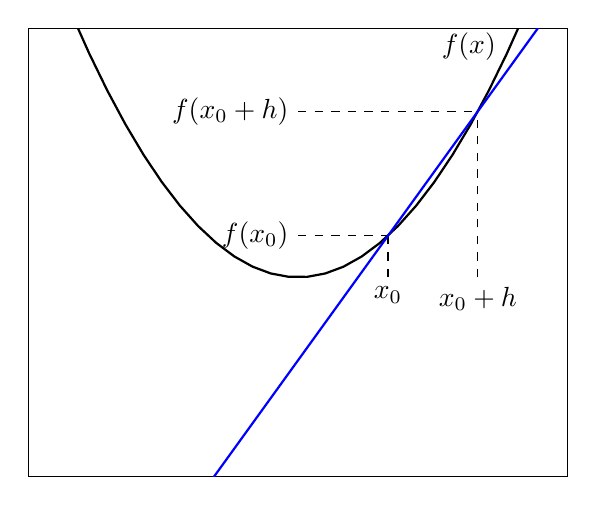
\begin{tikzpicture}
\begin{axis}[xmin=-1.5,xmax=1.5,ymin=-1.2,ymax=1.5,ticks=none]
	\addplot[thick, samples=100] {x^2};
	\draw[dashed] (axis cs:0.5,0) -- (axis cs:0.5,0.25);	
	\node[below] at (axis cs:0.5,0){$x_0$};
	\draw[dashed] (axis cs:0,0.25) -- (axis cs:0.5,0.25);	
	\node[left] at (axis cs:0,0.25){$f(x_0)$};
	
	\draw[dashed] (axis cs:1,0) -- (axis cs:1,1);	
	\node[below] at (axis cs:1,0){$x_0+h$};
	\draw[dashed] (axis cs:0,1) -- (axis cs:1,1);	
	\node[left] at (axis cs:0,1){$f(x_0+h)$};
	
	\node[above left=3 pt] at (axis cs:1.2,1.2){$f(x)$};
	
	\addplot[thick,blue, samples=100] {1.5*x-0.5};
\end{axis}
\end{tikzpicture}
\caption{En sekant i punktet $x_0$}
\label{fig:Diff1et}
\end{minipage}
\begin{minipage}{0.49\textwidth}
 \centering
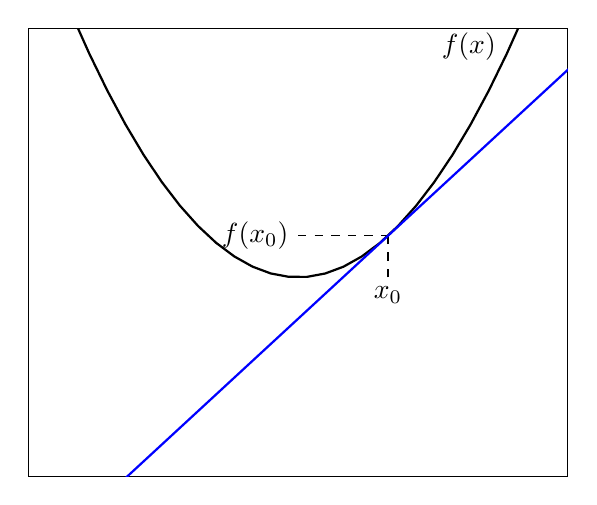
\begin{tikzpicture}
\begin{axis}[xmin=-1.5,xmax=1.5,ymin=-1.2,ymax=1.5,ticks=none]
	\addplot[thick, samples=100] {x^2};
	\draw[dashed] (axis cs:0.5,0) -- (axis cs:0.5,0.25);	
	\node[below] at (axis cs:0.5,0){$x_0$};
	\draw[dashed] (axis cs:0,0.25) -- (axis cs:0.5,0.25);	
	\node[left] at (axis cs:0,0.25){$f(x_0)$};
	
	\node[above left=3 pt] at (axis cs:1.2,1.2){$f(x)$};
	
	\addplot[thick,blue, samples=100] {x-0.25};
\end{axis}
\end{tikzpicture}
\caption{Sekanten når $h$ er tæt på $0$}
\label{fig:Diff1to}
\end{minipage}
\end{figure}

\paragraph*{Eksempler:}
\begin{enumerate}
\item Bestem differentialkvotienten af funktionen $f(x)=ax+b$ i $x_0$:

Vi indsætter funktionen i \eqref{eq:diff1et} og får
\begin{align*}
\lim_{h \to 0} \frac{f(x_0+h)-f(x_0)}{h}.
\end{align*}
Vi kan ikke umiddelbart tage grænsen, da vi så vil dividere med $0$. Derfor omskriver vi først og tager dernæst grænsen
\begin{align*}
\lim_{h \to 0} \frac{f(x_0+h)-f(x_0)}{h} &= \lim_{h \to 0} \frac{a(x_0+h)+b-(ax_0+b)}{h}\\
&= \lim_{h \to 0} \frac{ax_0+ah+b-ax_0-b)}{h} \\
&= \lim_{h \to 0} \frac{ah}{h} \\
&= \lim_{h \to 0} a \\
&= a.
\end{align*}
Dette viser, at $f'(x_0)=a$. Bemærk, at dette stemmer overens med at vi tidligere sagde at hældningen for en ret linje er $a$.
\item Vis at funktionen $f(x)=\vert x \vert$ ikke er differentiabel i $x=0$:

Vi husker, at $f(x)=\vert x \vert$ betyder at
\begin{align*}
f(x) = \begin{cases}
x & \textup{hvis } x \geq 0, \\
-x & \textup{hvis } x <0.
\end{cases}
\end{align*}
Vi betragter grænsen fra venstre og får
\begin{align*}
\lim_{h \to 0^-} \frac{f(0+h)-f(0)}{h} &= \lim_{h \to 0^-} \frac{\vert 0 + h \vert - \vert 0 \vert}{h} \\
&= \lim_{h \to 0^-} \frac{\vert h \vert}{h} \\
&= \lim_{h \to 0^-} \frac{-h}{h} \\
&= \lim_{h \to 0^-} -1 \\
&= -1,
\end{align*}
hvor den tredje lighed gælder fordi $h$ nærmer sig $0$ fra venstre, hvilket betyder at $h$ er negativ og så er $\vert h \vert = -h$.

Dernæst kigger vi på grænsen fra højre og får
\begin{align*}
\lim_{h \to 0^+} \frac{f(0+h)-f(0)}{h} &= \lim_{h \to 0^+} \frac{\vert 0 + h \vert - \vert 0 \vert}{h} \\
&= \lim_{h \to 0^+} \frac{\vert h \vert}{h} \\
&= \lim_{h \to 0^+} \frac{h}{h} \\
&= \lim_{h \to 0^+} 1 \\
&= 1,
\end{align*}
hvor den tredje lighed gælder fordi $h$ nærmer sig $0$ fra højre, hvilket betyder at $h$ er positiv og dermed har vi $\vert h \vert =h$.

Da grænsen i $0$ fra højre ikke er lig med grænsen i $0$ fra venstre, giver differentialkvotienten ikke mening i $0$, og dermed er $f$ ikke differentiabel i $0$.
\end{enumerate}

\paragraph*{Regneregler:}
Vi har følgende regneregler for når man skal finde differentialkvotienten for en funktion.
\begin{enumerate}
\item $(c \cdot f)'(x) = c \cdot f'(x)$, hvor $c \in \mathbb{R}$.

\item $(f\pm g)'(x) = f'(x) \pm g'(x)$.
\end{enumerate}
Der findes flere regneregler for at finde differentialkvotienter, som vi vil betragte de næste par kursusgange.
\paragraph*{Tabel over funktioner og deres differentialkvotient:}
Følgende er en tabel over de mest almindelige funktioner og deres differentialkvotienter. 

\begin{table}[h!]
\centering
\begin{tabular}{l !{\qquad} {c}!}
$f(x)$      & $f'(x)$  				\\ \toprule
$c$			& $0$ 					\\ \midrule
$x$			& $1$					\\ \midrule
$x^n$  		& $nx^{n-1}$				\\ \midrule
$\sqrt{x}$	& $\frac{1}{2\sqrt{x}}$	\\ \midrule
$\frac{1}{x}$& $-\frac{1}{x^2}$		\\ \midrule
$e^x$  		& $e^x$					\\ \midrule
$e^{cx}$  	& $ce^{cx}$				\\ \midrule
$a^x$  		& $a^x\ln a $			\\ \midrule
$\log_a x$ 	& $\frac{1}{x\ln a}$	\\ \midrule
$\ln x$ 	& $\frac{1}{x}$			\\ \midrule
$\cos x$  	& $-\sin x$				\\ \midrule
$\sin x$  	& $\cos x$				\\ \midrule
$\tan x$ 	& $1+\tan^2(x)$	\\ \bottomrule  
\end{tabular}
\caption{Udvalgte differentialkvotienter.}
\label{tab:Diff1et}
\end{table}

\paragraph*{Eksempler:}
\begin{enumerate}
\item Differentier funktionen $f(x)=3x^3$:

Vi benytter regneregel $1.$ og Tabel~\ref{tab:Diff1et} til at få
\begin{align*}
f'(x) = \frac{d}{dx} (3x^3) = 3 \frac{d}{dx} x^3 = 3 \cdot 3 x^{3-1} = 9x^2.
\end{align*}
\item Differentier funktionen $f(x)=\cos x$:

Vi benytter Tabel~\ref{tab:Diff1et} og får
\begin{align*}
f'(x) = \frac{d}{dx} \cos x = - \sin x.
\end{align*}
\item Differentier funktionen $f+g$ hvor $f(x)=e^{3x}$ og $g(x)= \ln x$:

Vi har fra regneregel $2.$ at vi kan differentiere de to funktioner hver for sig, og ved at benytte Tabel~\ref{tab:Diff1et} får vi at
\begin{align*}
(f+g)'(x) = f'(x) + g'(x) = \frac{d}{dx} e^{3x} + \frac{d}{dx}\ln x = 3e^{3x} + \frac{1}{x}.
\end{align*}
\item Differentier funktionen $f(x)=\ln(x^{\frac{1}{3}})$:

Vi kan ikke umiddelbart bruge Tabel~\ref{tab:Diff1et} til at differentiere $f(x)$ på denne form, men hvis vi i stedet omskriver funktionen ved hjælp af vores regneregler for den naturlige logaritme, så får vi
\begin{align*}
f(x) = \ln(x^{\frac{1}{3}}) = \frac{1}{3} \ln x.
\end{align*} 
Ved at benytte Tabel~\ref{tab:Diff1et} nu får vi at
\begin{align*}
f'(x) = \frac{d}{dx}\Big(\frac{1}{3} \ln x\Big)=\frac{1}{3} \frac{d}{dx}\ln x= \frac{1}{3} \cdot \frac{1}{x} = \frac{1}{3x}.
\end{align*}
\end{enumerate}
